\chapter{Experiments}
\label{ch:experiments}

This chapter details the experiments performed on the systems described in the previous chapters, contemplating from the front-end processes until the speaker modeling and the log-likelihood ratio test (see \equationref{score_of_X}). First, a description of the corpus is made. Then, explanations about the implementation are given. At last, the results are exhibited using the feature extraction process and the GMM techniques.

\section{Corpus}
\label{sec:corpus}

The database used in this work is the \emph{MIT Mobile Device Speaker Verification Corpus} (MIT-MDSCV), \refbib{Woo et. al.}{woo.park.hazen.2006}, a \textbf{corpus} designed to evaluate voice biometric systems of high mobility. All utterances were recorded using mobile devices of different models and manufacturers.

The corpus is composed of three sessions. The first, named ``Enroll 1", contains 48 speakers (22 females and 26 males), each with 54 utterances (names of ice cream flavors) of 1.8 seconds average duration, and is used to train an ASR system. The utterances were recorded in three different locations (a quiet office, a mildly noisy hallway, and a busy street intersection) as well as two different microphones (the built-in internal microphone of the handheld device and an external earpiece headset) leading to 6 distinct training conditions equally dividing the session. The second session, named ``Enroll 2", is similar to the first with a difference in the order of the spoken utterances, and is used to test the enrolled speakers. The third session, named ``Imposters", is similar to the first two, but with 40 non-enrolled speakers (17 females and 23 males), and is used to test the robustness of the ASR system (imposters should be rejected). \tableref{corpus-division} summarizes the division of the corpus.

\begin{table}[h]
    \small
    \centering
    \begin{tabular}{|l|c|c|}
    \hline
    \multicolumn{1}{|c|}{{\bf Session}} & {\bf Training} & {\bf Test} \\ \hline
    Enroll 1                            & {\bf X}        & {\bf }     \\ \hline
    Enroll 2                            & {\bf }         & {\bf X}    \\ \hline
    Imposter                            & {\bf }         & {\bf X}    \\ \hline
    \end{tabular}
    \caption{Corpus divided in training and test sets.}
    \label{tab:corpus-division}
\end{table}

All utterances are recorded in uncompressed WAV files using a single channel. For each utterance record there is a correspondent text file containing pertinent information, such as speaker who produced it, microphone used, location where the utterance was recorded, the spoken message content and etc. (see \tableref{utterance-info}).

Despite being a base for speaker verification systems, in this paper MIT-MDSCV is also used for speaker identification experiments. The difference is that only ``Enroll 1" and ``Enroll 2" are used, for training and test respectively. In an ideal identification system all utterances from ``Enroll 2" are correctly identified and in an ideal verification system the false detection and false rejection rates are zero.

\begin{table}[h]
    \small
    \centering
    \begin{tabular}{|l|c|}
    \hline
    {\bf Speaker}    & f00              \\ \hline
    {\bf Session}    & 1                \\ \hline
    {\bf List}       & female\_list\_3a \\ \hline
    {\bf Gender}     & female           \\ \hline
    {\bf Location}   & Office           \\ \hline
    {\bf Microphone} & Headset          \\ \hline
    {\bf Phrase}     & karen livescu    \\ \hline
    \end{tabular}
    \caption{Information from first utterance of first speaker in session ``Enroll 1".}
    \label{tab:utterance-info}
\end{table}

\section{Coding and Data Preparation}
\label{sec:coding-and-data-preparation}

The systems described throughout the paper were implemented in the Python programming language, version 3.4.3, and the frameworks NumPy 1.8.1 and SciPy 0.14.0 were used to perform most of the calculations as matrices. Also, Matplotlib 1.4 was used to plot the results as figures. All codes can be found in \url{github.com/embatbr/tg} and are free to be used, since properly referenced.

The implementation is divided in 6 modules. Module \textbf{features} contains codes to execute the feature extraction through the MFCC algorithm (see \chapterref{feature-extraction}). Each stage is executed by a different function. The main function joins all stages, receiving a speech signal in waveform and delivering a matrix of features over frames. The GMM is implemented in module \textbf{mixtures} as a class containing methods for training usign EM algorithm and for bayesian adaptation (see \sectionref{adapted-gmm}). The module also contains functions to execute the \emph{k-means} clustering, used during the GMM creation. Functions to extract the features from MIT-MDSCV and to read groups of feature data (from a single speaker, from a background and etc.) are present in module \textbf{bases}. The module \textbf{main}, as the name denounces, is filled with functions to execute every functionality needed. Through command lines it is possible to extract MFCCs from the base, train and adapt models, identify or verify speakers, and calculate rates and draw curves. Module \textbf{show} is aimed to generate figures to fill the previous chapters (mostly chapters \chapterrefcomp{feature-extraction} and \chapterrefcomp{gmm}). At last, module \textbf{common} contains useful constants and functions shared by the other modules.

\subsection{Parameters}

The MFCCs extracted used a filterbank of size 26, maintaining only the first 19 features, and deltas of order 0, 1 and 2, leading to MFCCs with final feature number of 19, 38 and 57, respectively. Before any delta calculation take place, the energy appending and CMS steps are performed. The relevance factor $r$ has a default value of 16 for all combinations of adaptations.

All speakers are modeled using SSGMMs with sizes ($M$s) 8, 16, 32, 64 and 128, each divided in 4 types of environment configuration: quiet office, mildly noisy hallway, busy street intersection and all three together. This leads to 48 speakers $\times$ 5 $M$s $\times$ 4 environments $\times$ 3 delta orders $=$ 2880 trained SSGMMs. The UBM is a combination of a trained male UBM and a trained female UBM (see \figureref{ubm-diagram}b), for all sizes of mixtures, types of environments and orders of delta, totaling 60 models. Each one of the 7 combinations of SSAGMM also contains 2880 models. Adding the Single Speaker Fractional Gaussian Mixture Models (SSFGMMs) for all 5 values of $r$ (1, 0.99, 1.01, 0.95 and 1.05), the total number of trained models is 37500.

\subsection{Algorithmic Issues}

According to \refbib{Reynolds}{reynolds.1995c}, different methods of initialization lead to different local maxima reached by the EM algorithm. Following the approach used in the referenced paper, in this work the models are generated randomly selecting the means and executing a single iteration \emph{k-means} to initialize the means, nodal variances and weights. A complete k-means (iterate until the clusters stop changing) during the initialization followed by EM training leads to a similar result, making the choice of single iteration k-means in the initialization the logical decision.

During the M-step of the EM algorithm, some variances may have their values decreased significantly. This represents a degeneration of the model, occuring when the size of mixture increases more than needed to represent the data or when the data is insufficient to train the model, \refbib{Reynolds}{reynolds.1995c}. This issue occurred in SSGMMs with 64 or 128 gaussians and UBMs with 128 gaussians. To prevent the degeneration, the EM algorithm receives a constraint: when the variance $\sigma^2$ is lower than a minimum variance $\sigma_{min}^2 = 0.01$, $\sigma_{min}^2$ is assigned to $\sigma^2$. This test is made in every iteration and provides more robustness to the ASR system (correct the degradation when it occurs, avoiding error propagation).

\section{Experiments and Results}
\label{sec:experiments-and-results}

Using the models trained (see previous section), two types of experiments were performed. The first, speaker identification in open set (see \sectionref{speaker-identification}), was executed using SSGMMs and SSFGMMs. Identification through SSGMM is an experiment known since \refbib{Reynolds}{reynolds.1992} was published in 1992, with countless revisions proving its correctness. Conversely, identification through SSFGMM (see \sectionref{frac-gmm}) is a technique never tried before and for that reason FGMM was used in speaker identification to validate the idea before further experiments. At the end SSGMM and SSFGMM were compared. The second type, speaker verification, was executed using SSGMMs and SSAGMMs, providing false detection and false rejection rates. The verification through SSAGMM was executed using all combinations of adaptations. Finally, a comparison between SSGMM and SSAGMM was performed.

The metrics used for evaluation differ according to the type of ASR system studied. For identification in closed set the interest is in know how well the system correctly identify an enrolled user. The logical way is by analyzing the success rate (the closer to 100\% the better). For verification, the major concern for the system designer is to avoid misclassification. The perfect point of operation is when false detection and false rejection rates are equal (Equal Error Rate, EER), used to evaluate the correctness of the system.

In the experiments performed, all 54 utterances from each speaker were tested against any one of the models created and trained for each environment configuration. The first, \textbf{office}, is a noise free environment. The second, \textbf{hallway}, presents a moderate level of noise. The third, \textbf{intersection} is a very lound environment. The last is a combination of all three previous environments, providing a model trained with different levels of noise. This approach allows a more refined analysis of the system's response to background noise.

\subsection{Speaker Identification using SSGMM}

As shown in \sectionref{speaker-identification}, \equationref{speaker_identification}, given a set $\dvec{\lambda} = \{\lambda_1, ..., \lambda_S\}$ of SSGMMs, a sequence of features $\boldsymbol{X}$ is assigned to a speaker $\mathcal{S}_i$, represented by a model $\lambda_i$ of $\dvec{\lambda}$, if $\postpdf{\boldsymbol{X}}{\lambda_i}$ is greater than all $\postpdf{\boldsymbol{X}}{\lambda_j}$, for $\lambda_j \in \dvec{\lambda}$ and $j \ne i$.

In this study, \equationref{speaker_identification} is used for all 54 speech signals of each enrolled speaker. The signals used are in session ``Enroll 2", as described in \sectionref{corpus}. The number of tests is 54 utterances $\times$ 48 enrolled speakers $\times$ 4 environment configurations $\times$ 5 sizes of mixture, totaling 51840. Tables \tablerefcomp{identify_speakers_mit_19_0}, \tablerefcomp{identify_speakers_mit_19_1} and \tablerefcomp{identify_speakers_mit_19_2} show the speaker identification success rates (in percent) for delta orders equal to 0, 1 and 2, respectively.

\begin{table}[h]
    \footnotesize
    \centering
    \begin{tabular}{|c|c|c|c|l|}    
    \hline
    {\bf M} & {\bf Office} & {\bf Hallway} & {\bf Intersection} &     \multicolumn{1}{c|}{{\bf All}} \\ \hline
    {\bf 8} & 41.55 & 52.66 & 42.48 & 64.66 \\ \hline
    {\bf 16} & 46.76 & 55.79 & 45.64 & 72.65 \\ \hline
    {\bf 32} & 50.08 & 58.68 & 47.53 & 77.93 \\ \hline
    {\bf 64} & 50.08 & 57.52 & 47.22 & 80.52 \\ \hline
    {\bf 128} & 47.84 & 52.93 & 44.48 & 81.21 \\ \hline
    \end{tabular}
    \caption{Identification rates for $\Delta = 0$.}    
    \label{tab:identify_speakers_mit_19_0}
\end{table}

\begin{table}[h]
    \footnotesize
    \centering
    \begin{tabular}{|c|c|c|c|l|}    
    \hline
    {\bf M} & {\bf Office} & {\bf Hallway} & {\bf Intersection} &     \multicolumn{1}{c|}{{\bf All}} \\ \hline
    {\bf 8} & 44.41 & 53.28 & 43.98 & 66.20 \\ \hline
    {\bf 16} & 50.58 & 61.30 & 50.81 & 78.12 \\ \hline
    {\bf 32} & 53.78 & 65.20 & 53.09 & 85.03 \\ \hline
    {\bf 64} & 54.21 & 64.43 & 52.43 & 87.85 \\ \hline
    {\bf 128} & 52.82 & 59.53 & 49.42 & 88.46 \\ \hline
    \end{tabular}
    \caption{Identification rates for $\Delta = 1$.}    
    \label{tab:identify_speakers_mit_19_1}
\end{table}

\begin{table}[h]
    \footnotesize
    \centering
    \begin{tabular}{|c|c|c|c|l|}    
    \hline
    {\bf M} & {\bf Office} & {\bf Hallway} & {\bf Intersection} &     \multicolumn{1}{c|}{{\bf All}} \\ \hline
    {\bf 8} & 45.02 & 56.06 & 46.60 & 68.56 \\ \hline
    {\bf 16} & 50.62 & 62.81 & 50.89 & 79.32 \\ \hline
    {\bf 32} & 54.44 & 65.39 & 54.98 & 85.69 \\ \hline
    {\bf 64} & 56.33 & 63.93 & 54.67 & 89.54 \\ \hline
    {\bf 128} & 52.47 & 62.00 & 51.08 & 89.97 \\ \hline
    \end{tabular}
    \caption{Identification rates for $\Delta = 2$.}    
    \label{tab:identify_speakers_mit_19_2}
\end{table}


As seen in the tables above and in \figureref{identification-curves-speakers}, for the fourth environment configuration (all) the success rates increase with $M$, while for the other three (office, hallway and intersection) they reach a maximum value at $M = 32$. As explained in the previous section, SSGMMs suffered degeneration due to a decrease in the values of variances for 64 and 128 gaussians. A higher value of $M$ led to higher misrepresentation of the samples by the SSGMM, seen in the lower values $M = 64$ presents compared to the values of $M = 128$. The exception to this ``rule" is seen when all environments are used in the training. This may be explained due to the higher number of samples (each speaker has 18 utterances recorded in each environment, leading to all 54 speech signals being used to train the model). Also as expected, when all environments are present, the SSGMM represents different levels of background noise, what produces a more robust modeling.

\begin{figure}[ht]
    \centering
    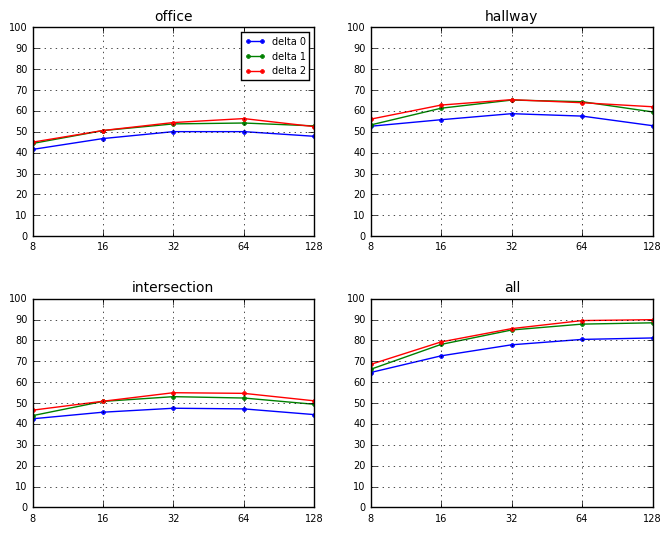
\includegraphics[width=\textwidth]{identification-curves-speakers}
    \caption{Identification success rates for enrolled speakers using different orders of delta.}
    \label{fig:identification-curves-speakers}
\end{figure}

%\subsection{Speaker Identification using SSFGMM}

%\subsection{Comparison between SSGMM and SSFGMM}

%\subsection{Speaker Verification using SSGMM}

%\subsection{Speaker Verification using SSAGMM}

%\subsection{Speaker Verification using SSFGMM}

%\subsection{Comparison between SSGMM and SSAGMM}

%\subsection{Comparison between SSGMM and SSFGMM}